\documentclass[10pt,a4paper]{article}
\usepackage[utf8x]{inputenc}
\usepackage[T1]{fontenc}
%\usepackage{stringenc} % for grffile
\usepackage{ucs}
\usepackage{amsthm} %numéroter les questions
\usepackage[english]{babel}
\usepackage{datetime}
\usepackage{xspace} % typographie IN
\usepackage{hyperref}% hyperliens
\usepackage[all]{hypcap} %lien pointe en haut des figures
\usepackage[english]{varioref} %voir x p y
\usepackage{fancyhdr}% en têtes
%\input cyracc.def
\usepackage[]{graphicx} %include pictures
%\usepackage[encoding,inputencoding=utf8,filenameencoding=utf8]{grffile}
%\usepackage[extendedchars,inputencoding=latin1,filenameencoding=latin1]{grffile}
\usepackage[siunitx ]{circuitikz}
\usepackage{gnuplottex}
\usepackage{ifthen}
\graphicspath{{./figures/}}
%\usepackage{array}
\usepackage{amsmath}
\usepackage[]{xcolor}
\usepackage{tikz}
\usepackage{tikz-timing}
\usetikzlibrary{scopes}
\usetikzlibrary{backgrounds}
\usepackage{listings}
\usepackage{enumitem}
\usepackage[top=1 in, bottom=1 in, left=1.3 in, right=1 in]{geometry} % Yeah, that's bad to play with margins
\usepackage[]{pdfpages}
\usepackage{pdflscape}
\usepackage[]{attachfile}
%\usepackage{colortbl}
%\usepackage{multirow}
\usepackage{booktabs}
\usepackage{makecell}
\usepackage[ ]{subfig}
%\usepackage{rotating}
\usepackage{upgreek}
\usepackage[normalem]{ulem}

\newdateformat{mydate}{2018--2019}%hack pour remplacer \THEYEAR

%cyr
%\newcommand\textcyr[1]{{\fontencoding{OT2}\fontfamily{wncyr}\selectfont #1}}
\renewcommand{\marginpar}[1]{} %surcharge pour /marginpar

\newboolean{corrige}
%\setboolean{corrige}{true}%corrigé
\setboolean{corrige}{false}% pas de corrigé

\newboolean{annexes}
%\setboolean{annexes}{true}%annexes
\setboolean{annexes}{false}% pas de annexes

\newboolean{mos}
%\setboolean{mos}{true}%annexes
\setboolean{mos}{false}% pas de annexes

\usepackage{aeguill} %guillemets

%% fancy header & foot
\pagestyle{fancy}
\lhead{[ELEC-H-410] Real-Time systems Lab n° 1: \rtos}
\rhead{\mydate\today\\ page \thepage}
\chead{\ifthenelse{\boolean{corrige}}{Corrigé}{}}
\cfoot{}
%%

\pdfinfo{
    /Author (BEAMS)
    /Title (Lab n° 1 ELEC-H-410, uCOS-II)
    /ModDate (D:\pdfdate)
}

\hypersetup{
    pdftitle={Lab n° 1 [ELEC-H-410] Real-Time systems},
    pdfauthor={BEAMS},
    pdfsubject={FreeRTOS}
}

\theoremstyle{definition}% questions pas en italique
\newtheorem{E}{\color{blue}Exercise}[] % numéroter les questions [section] ou non []

\newcommand{\reponse}[1]{% pour intégrer une réponse : \reponse{texte} : sera inclus si \boolean{corrige}
	\ifthenelse {\boolean{corrige}} {\paragraph{Réponse :} #1} {}
 }

\newcommand{\addcontentslinenono}[4]{\addtocontents{#1}{\protect\contentsline{#2}{#3}{#4}{}}}

\newcommand{\on}[1]{\operatorname{#1}}

\newcommand{\reg}[1]{\texttt{reg#1}}

\newcommand{\rtos}{FreeRTOS}

\newcommand{\kw}[1]{\texttt{#1}}

\setlength{\parskip}{1ex plus .5ex minus .5ex} % espacement entre paragraphes
\setlength{\parindent}{0 ex plus 0ex minus 0 ex} % retrait en début de §

\def\labelitemi{--}
\setlist{parsep=0pt,itemsep=0pt,style=standard,leftmargin=\parindent, align=left} % pas d'espace prohibitif entre les items
\setlist{nolistsep}

\newcolumntype{C}[1]{>{\centering\let\newline\\\arraybackslash\hspace{0pt}}m{#1}}

%\setlength{\tabcolsep}{0pt} %no extra space in cells to keep constant tabular width

\date{\vspace{-1cm}\mydate\today}
\title{\vspace{-2cm} Lab n° 1\\ Real-Time systems [ELEC-H-410]\\ Realization of an application under \rtos~\ifthenelse{\boolean{corrige}}{~\\Corrigé}{}}

%\author{\vspace{-1cm}}%\textsc{Yannick Allard}}


\lstdefinestyle{customasm}{
    % belowcaptionskip=1\baselineskip,
    % frame=L,
    % xleftmargin=\parindent,
    language=[x86masm]Assembler,
    basicstyle=\footnotesize\ttfamily,
    commentstyle=\itshape\color{purple!40!black},
    comment=[l]//,
}
\lstdefinestyle{customc}{
    belowcaptionskip=1\baselineskip,
    breaklines=true,
    frame=L,
    xleftmargin=\parindent,
    language=C,
    showstringspaces=false,
    basicstyle=\footnotesize\ttfamily,
    keywordstyle=\bfseries\color{green!40!black},
    commentstyle=\itshape\color{purple!40!black},
    identifierstyle=\color{blue},
    stringstyle=\color{orange},
}
\lstset{escapechar=@,style=customc}

\begin{document}

    % Introduce a new counter for counting the nodes needed for circling
    \newcounter{nodecount}
    % Command for making a new node and naming it according to the nodecount counter
    \newcommand\tabnode[1]{\addtocounter{nodecount}{1} \tikz \node (\arabic{nodecount}) {#1};}
    
    % Some options common to all the nodes and paths
    \tikzstyle{every picture}+=[remember picture,baseline]
    \tikzstyle{every node}+=[inner sep=0pt,anchor=base]
    \tikzstyle{every path}+=[thick, rounded corners]
    
    % for tikz pict
    
    \maketitle
    In order  for you to work remotely, we changed this year project into a game. The game simulates a pandemic situation, very much like the one we are seeing right now. As you have seen, real-time response is a critical component of handling a pandemic efficiently. 

It is by no means our intention to take the current epidemic lightly. However, we thought that this project assignment would allow to lighten the mood a little, as everyone's morale will also be taking a serious hit during this period of confinement. Keep your spirits high and make sure you give your courses your best (all of them, not just this one). We will need talented and bright engineers in the aftermath of this crisis.  

To play this game, you don't need any equipment other than the PSOC itself.
The game is entirely coded inside one FreeRTOS task (\textit{gameTask}).
It sends "events" and we ask you to make a code that will automatically respond to those "events".\\
Depending on your response time you will increase or not some variables.

\subsection*{Useful documentation:}
\begin{itemize}
    \item Official \rtos~ documentation: \url{https://www.freertos.org/Documentation/RTOS_book.html}
    \item Getting Started with PSoC 5LP: \url{https://www.cypress.com/file/41436/download}
    \item Video example on how to use the PSoC: \url{https://www.cypress.com/video-library/PSoC}
    \item The extension board schematics: \texttt{Extension\_PSoC.pdf}
		\item Getting started with the Logic Analyzer: \url{https://learn.sparkfun.com/tutorials/using-the-usb-logic-analyzer-with-sigrok-pulseview}
\end{itemize}

    
    
\section{First lab}
During this first lab, you will learn how to write a task under \rtos, to make it periodic and to assign
it a priority, in an intelligent way. The hardware will be composed of the PSoC and a logic analyser.

If you are not confident with C programming, read \texttt{C\_language\_for\_uC.pdf}.

Principles of the logic analyser are explained in the chapter 9; as well as in Lab 0.

\subsection{Creation of a task under \rtos~}

    A task is a succession of instructions doing a specific operation. Contrary to a function, a task cannot
    return a value. Moreover you do not have any direct influence on the order of execution of the various tasks you create. Indeed, it is the operating system which is given the responsibility to schedule the tasks and thus to choose which task must be carried out at which time on the processor. \rtos~ is a preemptive RTOS based on fixed priorities that you assign to the tasks. The choice of those priorities is thus critical so that the system behaves as you wish. This is why the second part of this lab will be related to the wise choice of priorities.
    
    First, you will learn how to create a single simple task in \rtos~ and to initiate the execution of the
    operating system.

    % TODO Addapt
    {\color{red} Copy the project \verb!\ELEC-H-410\lab1\!\textbf{ex1\_blinky} to your computer} and open the project with \texttt{PSoC Creator}.

    \vbox{In the file main.c you will find the  \verb!main! function  (see Listing \ref{lst:listing 1}) in which are executed :
    \begin{itemize}
    \item the initialisation of \rtos: \kw{freeRTOSInit()}
    \item the creation of a task : \kw{xTaskCreate()}
    \item the starting of \rtos: \kw{vTaskStartScheduler()}
    \end{itemize}
    }

    This structure cannot vary. The operating system must indeed be initialised before any creation of task and at least one task must have been created before giving control to OS.
    
    For more details on the parameters sent during the creation of the task, refer to the Task Creation section of the documentation of \rtos\footnote{\url{https://www.freertos.org/a00125.html}}.
    %\newpage
    \begin{lstlisting}[caption={Function main.c}, label={lst:listing 1}]
    #include "project.h"
    // [...]
    
    TaskHandle_t taskHandler;
    
    int main(void)
    {
        freeRTOSInit();
        
        // [...]
        
        // Task creation
        xTaskCreate( task,
                     TASK_NAME,
                     TASK_STACK_SIZE,
                     NULL,
                     TASK_PRIORITY,
                     &taskHandler );
    
        // [...]
        
        // Start FreeRTOS
        vTaskStartScheduler();     
        
        for(;;)
        {
            // This line of code is unreachable
        }
    }
    \end{lstlisting}
    %\marginpar{OK add caption and refr to listing} done

\subsection{How to write a task}
    Adding tasks to the OS is very easy:
    \begin{itemize}
        \item The task must be written like a function which returns nothing (\kw{void}).
        \item The task must contain an infinite loop.
        \item A task must always call at least one of the services of \rtos~that will make the task \mbox{``waiting"} such as  \kw{vTaskDelay()} or \kw{vTaskSuspend()}.
    \end{itemize}
    Since \rtos~is preemptive, the currently running task has got the highest priority among all “ready” tasks, hence if no event occurs (like an ISR making a higher priority task ready or the current task giving the control back to the scheduler) no other tasks will ever run.

    \begin{lstlisting}[caption={Basic task example}, label={lst:listing 2}]
    void task1( void *data )
    {
        // [...] init code, variable declaration
        
        for(;;)
        {
            // [...] task code
            vTaskDelay(10); // Ask the RTOS to put task1 in "waiting"
                            // state for at least 9 ticks
        }
    }
    \end{lstlisting}

\newpage
\subsection{Put a task to sleep for some time}
    Sometimes, it is necessary to let a task sleep for a while (maybe the job is complete, the task needs some resource/data not available yet to complete its job\dots)% \marginpar{reformuler}

    To let a task sleep in ``waiting" state for some time, one might call the \kw{vTaskDelay(uint32\_t ticks)} function; The parameter \kw{ticks} is an unsigned 32bit integer\footnote{ranging from 0 to $ 2^{32} - 1 $} which determines the number of ticks during which the task will sleep. The timer creating the periodic interrupts has been configured for a frequency of $ 1 $~Hz, hence $1$ tick = $ 1 $~ms. More precisely the task will sleep at least (\kw{ticks-1}), if you want to be sure to sleep during 1 tick you should specify \kw{ticks=2}. To demonstrate that, draw a chronogram of tick interrupts and imagine where the call \kw{vTaskDelay()} could occur.

    \E{\label{ex:1}
        Modify the task in the \kw{blinky} project to lights a LED of the $ \mu C $ board at a frequency of $ 1 $~Hz.
        Then create a second task that will lights another LED at a frequency of $ 2 $~Hz.

        To change the state of the the LED $ D1 $ you may use \kw{LED1\_Write(1u);}, this is an API\footnote{Application Programming Interface} automatically generated by PSoC Creator. Peripherals are declared in the TopDesign tab. Check the datasheet of LED1 to see what other API you could use.
    }{}

\subsection{Creation of periodic tasks}
    In Exercise \ref{ex:1}, you have created a periodic task, \textit{i.e.} a task executing forever at regular intervals. In most industrial applications, those tasks are frequent and the periodicity should be realised with a good precision (see example of PI controller in chapter 3 of the course).

    Open the project \kw{Periodicity}.

    You will find 4 tasks in this example:
    \begin{itemize}
        \item \kw{task1} which should have a period of 10ms;
        \item \kw{task2} which should have a period of 50ms;
        \item \kw{task3} which should have a period of 100ms.
    \end{itemize}

    \E{
        Scheduling verification. We will use the logic analyser to verify if your task is scheduled correctly in the RTOS.
        \begin{itemize}
            \item Switch the logic analyser on and launch the display interface on the PC.
            \item Start your program \kw{Periodicity} on the microcontroller and launch a first data acquisition with the logic analyser.
            \item Observe preemptions of certain tasks when a higher priority task is active (see signals \kw{input1}, \kw{input2} and \kw{input3} whose value is 1 when the tasks \kw{task1}, \kw{task2} and \kw{task3} are respectively active, \textit{i.e.}, between its first instruction until its completion).
            \item Use the logic analyser to measure the real period of real activation of each task. Are they exactly in conformity with the desired periods? Identify 2 causes of these errors.
        \end{itemize}
    }{}\reponse{
        Tasks are delayed by a complete period at the end of each iteration without taking into account the time spent inside the loop. 
        Plus, the OS which has a higher priority preempt the task when needed.
    }

    \subsubsection{Use of \kw{xTaskGetTickCount()}}
        \rtos~provides the \kw{xTaskGetTickCount()} function which returns a 32 bit integer (\kw{uint32\_t}) representing the number of ticks since the launching of OS.

        \E{
            Compute after how long this counter will overflow.
        }{}\reponse{
            $ 2^{32} - 1 $ ticks = 49.7 days
        }

        \E{
            Use \kw{xTaskGetTickCount()} in each task to compensate for the error over the period.
        }{}

    \subsubsection{Use of a software timer}

        It is possible to use software timers in \rtos. Those are used exactly in the same way as hardware timers, except that they are entirely managed by the operating system and that they are synchronised on the ticks of the system. The function \kw{xTimerCreate()} allows to create a software timer (see \rtos~ documentation for details) and \kw{xTimerStart()} to start it. When a timer expires, it calls a function whose pointer was given in the parameters.

        Open the project \kw{Timer}.
        You will find the same 4 tasks as in the previous example except that their period are generated by using three software timers.

        Functions \kw{vTaskSuspend()} and \kw{vTaskResume()} allow to suspend and restart the execution of a specific task.

        \E{
            Check with the logic analyser that the periods are strictly respected.
        }{}

        This method for creating periodic task gives very precise results. However, it is rather heavy and should therefore be used when this precision is absolutely required.

        \E{
            Create a new timer which switches a LED on after 5s. There is no need to write a complete task for this exercise.
        }{}

    \subsubsection{Choice of the priorities}

        As explained earlier, the choice of the priorities of the task is the only tool at our disposal to help the operating system to choose which task must be running at which time. To be convinced of the importance of a judicious choice of these priorities, we will look at a simple example.
        \E{Open the project \kw{Priorities}.}{}
        \begin{itemize}
            \item The task \kw{task1} should run every 1ms
            \item The task \kw{task2} should run every 100ms
            \item Check the behaviour of the tasks with the logic analyser.
            \item Reverse the priorities of \kw{AppTask1} and \kw{AppTask2} and reverify what occurs.
            \item By comparing the periods of each task and the priorities assigned, which systematic rule of assignment can you deduce?
            \item How is called this method to assign the priorities?
            \item What happens when tasks have relative deadlines different from their periods?
            \item Which scheduling algorithm would you use if you could assign priorities directly to jobs instead of tasks?
        \end{itemize}

    
    \vfill
    \footnotesize{
        Found an error? Let us know: \url{https://github.com/BEAMS-EE/ELECH410/issues}
    }
    
    \newpage
    \appendix

\section{The \textit{Asix Sigma2} logic analyser}
\label{ap:la}

The Asix Sigma2 logic analyser is like:\\ 
\begin{center}
    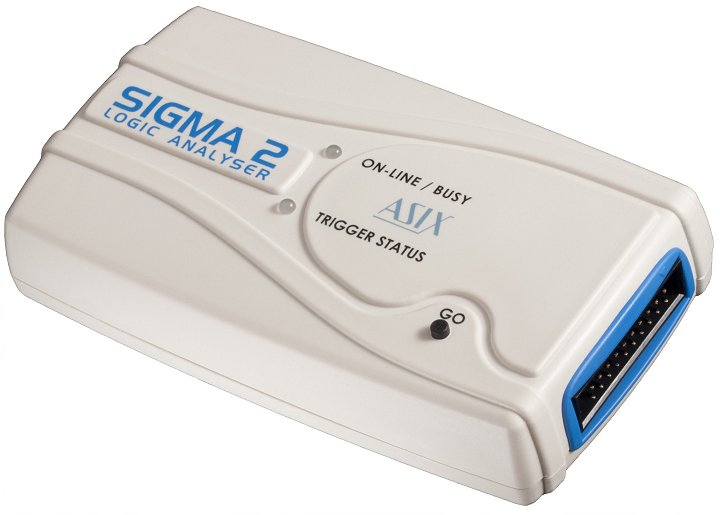
\includegraphics[width=4cm]{sigma2_720x515.jpg}
\end{center}

\subsection{Electrical connections to the Explorer 16 board}
    Connect the analyser to the extension board with the numbered ribbon cable following this scheme:
    \begin{center}
        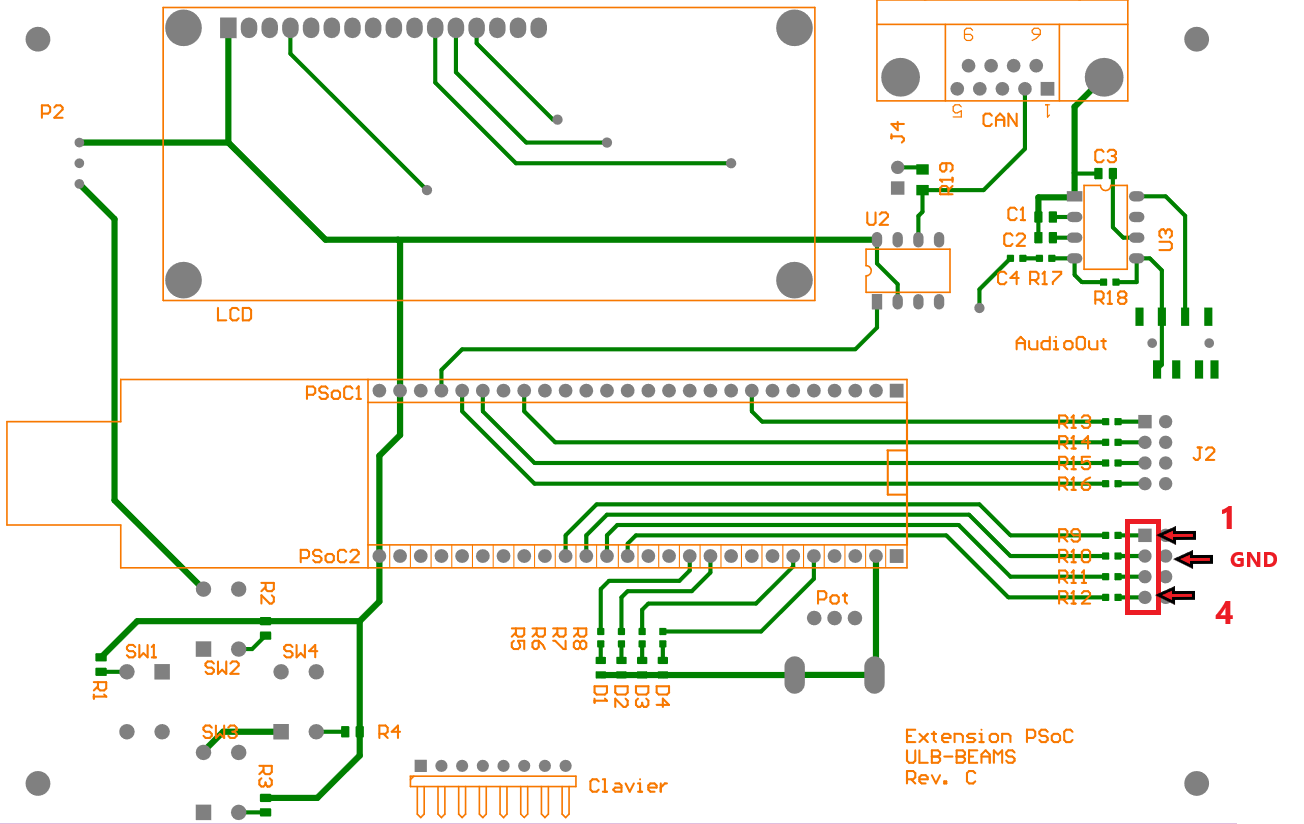
\includegraphics[width=0.7\textwidth]{analyserConnection.png}
    \end{center}

\subsection{Software on the computer}
    The software interface of the logic analyser looks like:
    \begin{center}
    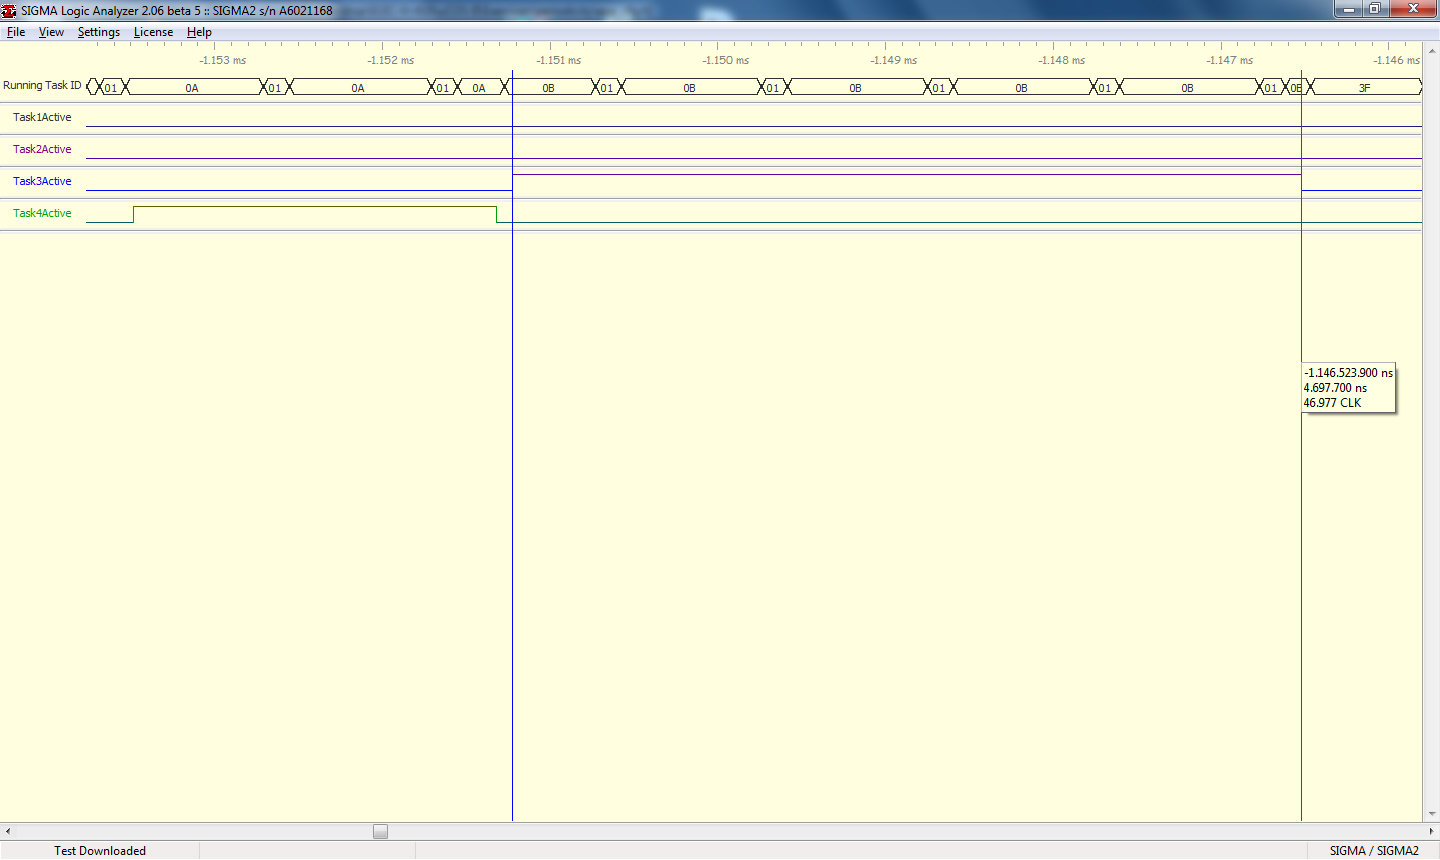
\includegraphics[width=13cm,trim= 0 100mm 0 0,clip]{Print_Screen_Logic_Analyzer.png}
    \end{center}

\subsection{Basic measurements}
    The red line on the screen is a cursor showing the time and values of signals in the main window. To place a marker (blue line), press space. If you move your cursor, the difference between the marker and the cursor will show in a tooltip.

    The first acquisition must be launched by software. Following acquisitions can be done using the ``go" button of the analyser.


\end{document}
